\documentclass{article}

%% Language and font encodings
\usepackage[english]{babel}
\usepackage[utf8x]{inputenc}
\usepackage[T1]{fontenc}
\usepackage[numbers]{natbib}
\bibliographystyle{plainnat}
\usepackage{booktabs}

%% Sets page size and margins
\usepackage[a4paper,top=3cm,bottom=2cm,left=3cm,right=3cm,marginparwidth=1.75cm]{geometry}

%% Useful packages
\usepackage{amsmath}
\usepackage{amssymb}
\usepackage{graphicx}
\usepackage[colorlinks=true, allcolors=blue]{hyperref}
\usepackage{setspace}
\usepackage{lineno}  % For reviewers
\usepackage{authblk}
\usepackage{blindtext}
\usepackage{fancyhdr}

% Use pretty font
\usepackage[scaled]{palatino}
\renewcommand\familydefault{\sfdefault} 
\usepackage[T1]{fontenc}

% big letter
\usepackage{lettrine}

\pagestyle{fancy}
\rhead{Homeostasis and oscillations}

% -----------------------------------------------------
% -----------------------------------------------------
% -----------------------------------------------------
\title{Homeostatic mechanisms may shape the type and duration of oscillatory modulation.}
\author[1,2,*]{Erik J. Peterson}
\author[2,3,4]{Bradley Voytek}

\affil[1]{Department of Psychology. Carnegie Mellon University, Pittsburgh, PA 15213}
\affil[2]{Department of Cognitive Science,~~~~~~~~~~~~~~~~~~~~~~~~~~~~~~~~~~~~~~~~~~~~~~~~~~~~~~~~~~~~~~~~~~~~~~}
\affil[3]{Neurosciences Graduate Program,~~~~~~~~~~~~~~~~~~~~~~~~~~~~~~~~~~~~~~~~~~~~~~~~~~~~~~~~~~~~~~~~~~~~}
\affil[4]{Hal{\i}c{\i}o\u{g}lu Data Science Institute, University of California, San Diego, 92093~~~~}
\affil[*]{Corresponding author: Erik.Exists@gmail.com~~~~~~~~~~~~~~~~~~~~~~~~~~~~~~~~~~~~~~~~~~~~~~~~~~}
\date{}                     %% if you don't need date to appear
\setcounter{Maxaffil}{0}
\renewcommand\Affilfont{\itshape\small}


\begin{document}
\maketitle
\linenumbers
% -----------------------------------------------------
% -----------------------------------------------------
% -----------------------------------------------------
\begin{abstract}
Neural oscillations are observed ubiquitously in the mammalian brain. However the stability of oscillations is highly variable. Some oscillations are \textit{tonic}, lasting for seconds or even minutes; others are unstable, appearing only as a single-cycle \textit{burst}. In a model of hippocampal neurons, we use numerical simulations to show how these different forms of rhythm stability can interact with activity-dependent homeostasis to profoundly alter the modulatory effect of neural oscillations. Under homeostasis, tonic oscillations that are synaptically excitatory have a paradoxical effect; they decrease excitability and desynchronizing firing. Tonic oscillations that are synaptically inhibitory--like those in a real hippocampus--fail to generate new action potentials and so provoke no homeostatic response. This may explain why the theta rhythm in hippocampus is synaptically inhibitory: inhibitory oscillations don't raise the firing threshold, as excitatory oscillations do, and so can preserve each cell's dynamic range. Based on these simulations, we also speculate that homeostasis may explain why excitatory intra-cortical and intra-layer oscillations often appear as bursts. In our model bursts minimally interact with the slow homeostasis time constant and so retain typical excitatory effects.\\
\end{abstract}

% -----------------------------------------------------
% -----------------------------------------------------
% -----------------------------------------------------
\noindent
\textsc{\textbf{New and Noteworthy}} In a model of hippocampal neurons we report a paradoxical result: Ca\textsuperscript{2+}-mediated homeostasis causes normally synchronizing AMPAergic oscillations to become inhibitory and desynchronizing. We conjecture this could be why the theta rhythm is inhibitory. In pyramidal cells GABA doesn't generate new action potentials and so provokes no homeostatic response. The intricate interplay of neuromodulators, like acetylcholine, with homeostasis is well known. The interplay between oscillations and homeostasis might be as complex, and as important.

\section*{Introduction}
\lettrine[loversize=0,nindent=0,realheight=true]{N}{} euromodulation and homeostasis are inter-linked but opposing phenomena. Modulation perturbs excitability, which we define as the propensity for a stimulus to elicit an action potential. Homeostasis acts to this quench perturbation, driving the excitability of the cell back to a biologically desirable set point \cite{LeMasson1993,Abbott1993}. While the interplay between chemical modulators and homeostasis has been studied for more than 20 years \cite{LeMasson1993,Abbott1993,Golowasch1999,Marder2014,Marder2015,Gutierrez2013}, the relationship between network-level synaptic modulations--like neural oscillations--and homeostasis is not well understood, on either theoretical or empirical grounds. Like neuromodulators, neural oscillations alter excitability and firing statistics. Uniquely, though, oscillations create synchronous windows of activity \cite{Lisman2013,Voytek2015}. Temporally grouping action potentials into windows improves signal to noise and increases the number of coincident firing events \cite{Chen2013,Zhou2015,Voytek2015a,Peterson2017}, driving learning at individual synapses \cite{Muller2011,Song2000,Markram1997}. 

We propose the same mechanisms that link homeostasis with chemical neuromodulation can also come into play during oscillatory modulation. After all, both kinds of modulation lead to tonic changes in spiking and in Ca\textsuperscript{2+} concentration, which can in turn drives changes to intrinsic homeostasis \cite{Liu1998}. 

To test this, we model activity-dependent intrinsic homeostasis in a feed-forward population of hippocampal pyramidal cells \cite{Siegel1994}. In this model homeostasis is mediated by a Ca\textsuperscript{2+}-dependent mechanism \cite{Golowasch1999,Marder2014,Marder2015,Gutierrez2013,OLeary2014} pioneered by LeMasson \cite{LeMasson1993,Abbott1993}. In this model, Ca\textsuperscript{2+} acts a sensor or proxy for tonic changes in the membrane voltage. To counter tonic changes in Ca\textsuperscript{2+} levels, the expression of ion channels is altered, returning the Ca\textsuperscript{2+} level to a predefined ``good'' value \cite{Golowasch1999,OLeary2013}. Following Siegel \cite{Siegel1994}, increases in Ca\textsuperscript{2+} lead to downregulation of Na\textsuperscript{+} and Ca\textsuperscript{2+} channels, and upregulation of fast K\textsuperscript{+} channels. To minimize the effect of homeostasis on the rise and fall of action potential dynamics, we also add a KCa channel which is not present in Siegel \citep{Siegel1994}. In real cells intrinsic homeostasis changes the expression level, membrane trafficking, and kinetics of ion channels. Here, these details are not directly simulated. Instead we mimic the net or bulk effect of all these changes by altering the maximum conductance of individual ionic channels, which are modelled using Hodgkin-Huxley terms \cite{LeMasson1993,OLeary2013,OLeary2014}.

Given that chemical modulators operate on both short and long times scales \cite{Marinelli2014,Marder2014,Cohen2015,Daw2002}, we examined two timescales of oscillation. We contrast the effects of shorts bursts of oscillation to long lasting tonic rhythms, both of which are observed {\textit{in vivo}}, and which may play different physiological, cognitive, and computational roles \cite{Lundqvist2016,vanEde2018}. We also explore how oscillation duration interacts with synapse type, examining both AMPA- or GABA-ergic oscillations.

In our highly simplified model of hippocampal cells, intrinsic homeostasis can profoundly alter the modulatory effect of neural oscillations. \textit{Tonic} excitatory modulation, paradoxically, generates a homeostatic response that increases the firing threshold. This suppresses excitability which, in turn, desynchronizes population activity. \textit{Bursts} of excitation, meanwhile, don't show homeostatic suppression, and may even benefit from a weak level of homeostasis. This is due the constant noisy background level input also present in the model, which homeostatic mechanisms help control. Inhibitory GABAergic oscillations, however, show little to no homeostatic effect, suggesting that inhibitory oscillations might better isolate any phase coding scheme from the stimulus-driven response. This is might be important, for example, in hippocampal phase-coding schemes of memory \cite{Lisman2013}. 

% -----------------------------------------------------
% -----------------------------------------------------
% -----------------------------------------------------
\section*{Results}
We study Ca\textsuperscript{2+}-mediated homeostasis in a feed-forward network, using single compartment neurons. We modulate this network using neural oscillations. Oscillations are simulated either as tonic, lasting for the entire experiment, or may as a burst at the end, where it overlaps with input stimulus (Figure~\ref{fig:f1}\textbf{a}). Input into the model has both a constant background level of noise (not shown), and a stronger stimulus that is delivered once homeostatic equilibrium is reached \cite{Barth2012} (Figure~\ref{fig:f1}). During this strong stimulus we measure the network's response and how population firing and synchrony are affected by homeostasis under different oscillatory regimes.

Each experiment began with an instantiation of a randomly generated feed-forward network. A single neuron from this network is depicted in Figure~\ref{fig:f1}\textbf{b}. This network is subjected to a range of modulatory and control conditions, including oscillatory strength, duration, and synapse type (AMPA or GABA). Each experiment lasted 20 seconds. In Figure~\ref{fig:f1}\textbf{c} we depict key aspects of model output during an experiment. 
In real systems, intrinsic homeostasis is thought to happen over minutes or days. However, simulation times that are hours or days long are not computationally feasible. As a result, we follow the field and study a model where Ca\textsuperscript{2+} dynamics happen with a 4-second half-life, denoted by $\tau_h$. Despite the radical difference between real and simulated time-scales, all that matters mathematically is that Ca\textsuperscript{2+} dynamics happen much slower than all the other synaptic/membrane dynamics. In practice, this means a timescale of $\tau_h > 4$ seconds is a reasonable first-order approximation \cite{Golowasch1999,Marder2014,Marder2015,Gutierrez2013,Marder2014,OLeary2014,LeMasson1993,Abbott1993}.

After homeostatic equilibrium is reached, we measure two features: the synchrony between action potentials (measured by the Kappa correlation) and changes in the excitability of the system (measured as a change in population firing rate). Both of which are defined in the \textit{Methods}. To ensure a consistent comparison between experiments, measurements were made over the same 4-cycle or 0.5 second period in all simulations.

% At the end of each experiment we measure three main features: synchrony between action potentials between different neurons, for a given type of modulation; changes in the excitability of the system--measured as a change in population firing rate--and; the ``computational error'' introduced by the combination of modulation and homeostasis. Error is defined as the mean squared error (MSE) measured by comparing spike-times recorded during experimental conditions to recordings made in identical populations simulated without modulation/homeostasis. To ensure a consistent comparison between experiments, measurements were made over the same 4-cycle period \emph{for all simulations}.

\begin{figure}
\centering
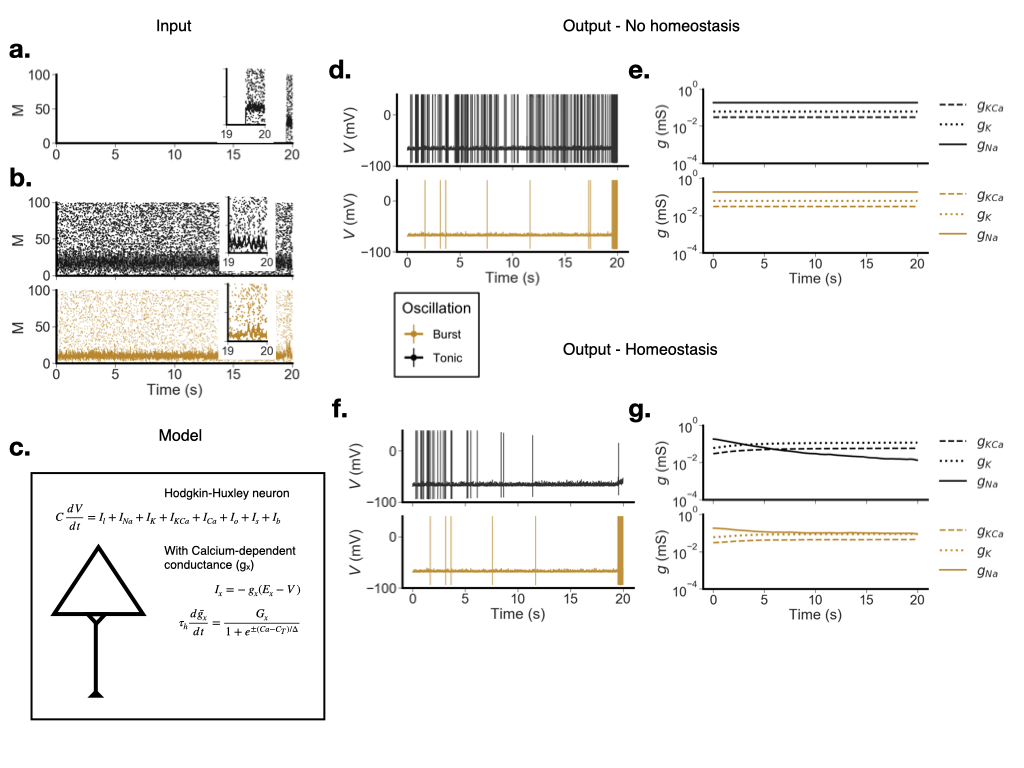
\includegraphics[width=0.9\textwidth]{fig1.png}
\caption{\label{fig:f1}
    Diagram of the model. \textbf{a}. Inputs into the model. Top panel depicts the stimulus, applied over the last 0.5 seconds of each simulated trial. Middle and bottom panels depict the two modes of oscillation we examined--tonic and bursting. 
    \textbf{b}. Illustration of a single model neuron, its major currents, its inputs (top arrow) and its output (bottom arrow).
    \textbf{c.} Examples of model output, including membrane potential (top panel), Ca\textsuperscript{2+} concentration, both observed (solid) and the homeostatic target (dotted line). The bottom panel in c. shows homeostatic dynamics beginning with trial onset, followed by a delay to equilibrium over 20 seconds. Note that there is no homeostatic response to stimulus onset at 19.5 seconds. Also note the log scale on the y axis in this panel.
}
\end{figure}

% -----------------------------------------------------------------------
\subsection*{Excitatory modulation.}
Homeostasis completely inverts the effect of tonic AMPAergic oscillatory modulation. To see how, first consider how the network responds to a tonic excitatory modulation without homeostasis. Without homeostasis, increasing the strength of the excitatory oscillation increases excitability, leading to an increase in the population firing rate. Additionally, the neuromodulatory effect of the oscillations is such that action potentials are grouped by oscillation phase, resulting in an increase in population synchrony (Figure \ref{fig:f2}\textbf{b}, black line). With homeostasis this pattern inverts. As excitatory oscillatory modulation strength increases, synchrony and excitability \emph{decreases} (Figure \ref{fig:f2}\textbf{c-d}). Homeostatic mechanisms in the model cause what \emph{should be} excitatory synchronizing modulation to become suppressive and desynchronizing. The stronger the oscillation, the more suppressive the result. By the time the oscillation is about half the strength of the stimulus (which we fix at a firing rate of 6 Hz) the stimulus is completely suppressed (\textit{i.e.}, the population firing rate approaches 0) (Figure \ref{fig:f2}\textbf{c}).

We compared the effect of tonic oscillation to short 4-cycle bursts of excitatory modulation, presented only during the stimulus. Here, the oscillation period is far too short to engage any additional homeostasis. This means that increases in oscillatory strength continue to increase population firing rate and synchrony (Figure~\ref{fig:f2}\textbf{e} and \textbf{f}).

Our model suggests tonic oscillations can profoundly alter coding properties of synaptically excitatory oscillations. This means that bursts of excitatory oscillation are \textit{qualitatively distinct} from their tonic counterparts. The decrease in excitability caused by tonic oscillation can be explained by a direct homeostatic change. Larger tonic oscillations lead to larger tonic increases in the membrane potential, which in turn raise Ca\textsuperscript{2+} levels. The homeostatic equations respond to this change Ca\textsuperscript{2+} by decreasing the conductance of the Na and Ca channels, and increasing the conductance of K and KCa channels (Eq~\ref{eq:dgdt}). The net effect of these dynamics is a increase in the firing threshold.

The inversion in Kappa seen in Figure~\ref{fig:f2}\textbf{d} as well as in \ref{fig:f4}\textbf{b}, is an artifact of the decrease in excitability; it's a low effect $N$ effect. As population spiking becomes more strongly suppressed the total number of spikes declines to the point where the bins used to calculate Kappa often contain no spikes. This in turn inflates Kappa values.

\subsection*{Inhibitory modulation.}
Both sustained tonic and bursting inhibitory oscillatory modulation do not lead to a homeostatic response in our model. In all cases, as oscillatory strength increases, population firing declines dramatically (grey lines in Figure \ref{fig:f2}\textbf{a-d} and light yellow lines in panel \textbf{e-f}).

% \subsection*{The synaptic nature of hippocampal theta.}

% \subsection*{Modulation, homeostasis, and error.}
% When increasing or decreasing the firing rate of a population, or its synchrony, action potentials can be added or re-arranged arbitrarily. We've suggested previously that an efficient modulator is one that adds or moves spikes as little as possible, while achieving a set level of effect \cite{Peterson2018a}. We define spike-time deviations introduced by modulation as an error compared to the original, unmodulated, population output (see Eq~\ref{eq:error} and \cite{Peterson2018a} for more background). We compare observed errors with and without homeostasis, for burst and tonic excitatory modulation. Given that synaptic inhibitory oscillatory modulation failed to trigger any homeostatic effects we don't include it in these analyses.

% Under homeostasis, tonic excitatory oscillations suppress the network responses to stimulation, leading to extremely high errors compared to an identical model simulated without homeostasis included (Figure~\ref{fig:f3}\textbf{a}). Bursts of excitatory oscillatory modulation, however, actually \textit{reduce} error compared to their non-homeostasis counterpart (Figure~\ref{fig:f3}\textbf{a}.). This decrease in error is driven by the baseline level of noise present in our stimulus model, which when input into the hippocampal population leads to a slight reduction in the excitability, this then positively interacts with the modulatory burst which ends more effective modulator compared to the baseline--homeostasis free--model.


\begin{figure}
\centering
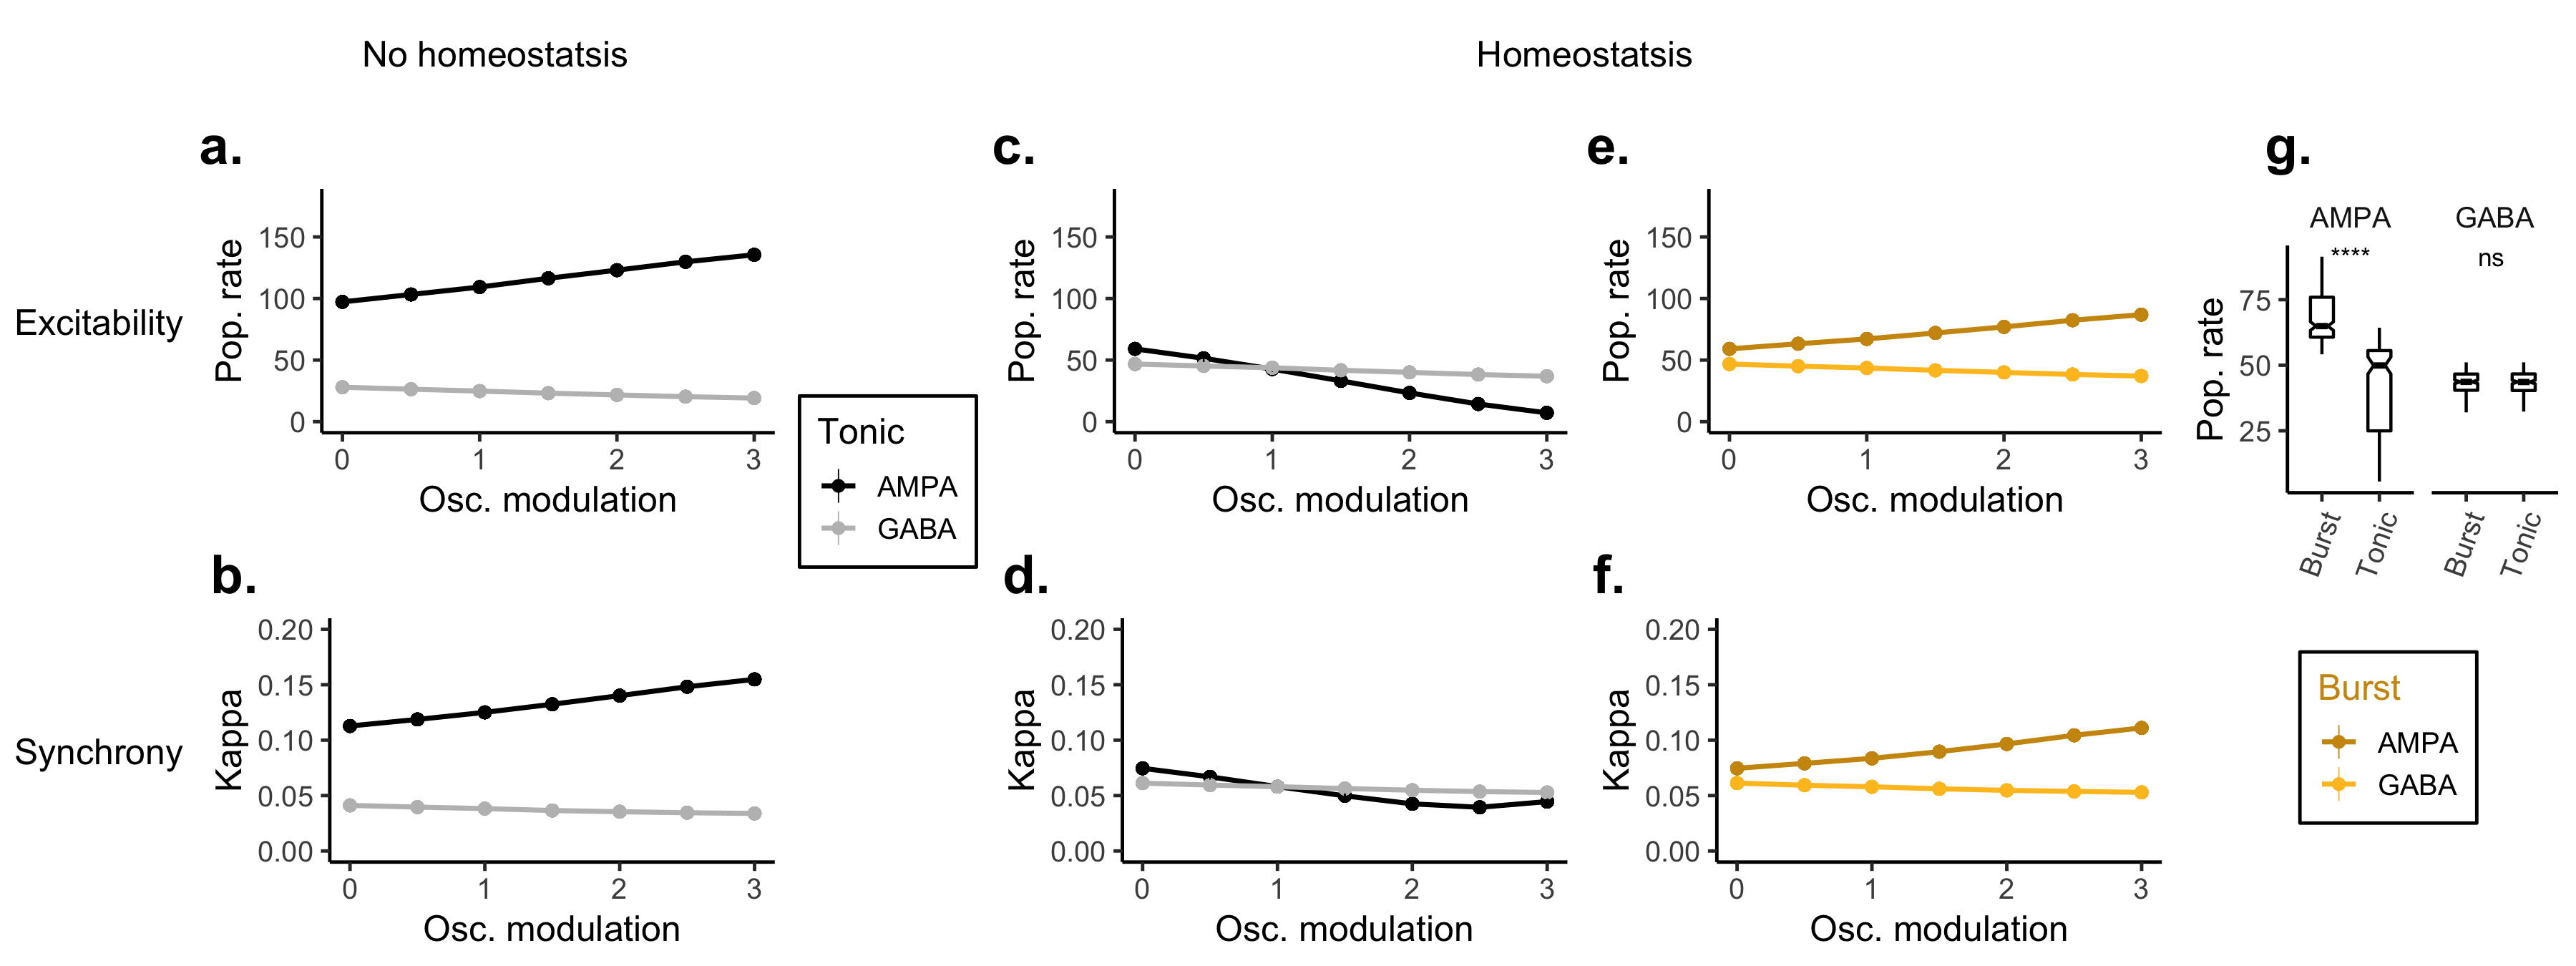
\includegraphics[width=1\textwidth]{fig2.png}
\caption{\label{fig:f2}
    The effect of oscillatory modulation on synchrony--which is measured using the Kappa correlation (Eq~\ref{eq:kappa})--and excitability, measured by the population firing rate. Tonic oscillations are shown in grey and black. Bursts are shown in light and dark yellow.
    \textbf{a.}-\textbf{b.} Increases in tonic modulation strength, without homeostasis. This is our reference condition. Top panel (a.) is the observed population firing rate averaged over the 0.5 second stimulus. Bottom (b.) is synchrony over the same period.
    \textbf{c.}-\textbf{d.} Same experiment as a-b but with Calcium-mediated homeostasis, showing how homeostasis with tonic AMPA oscillations reduces population firing and synchrony.
    \textbf{e.}-\textbf{f.} Burst modulation, presented during the stimulus period (4 cycles of oscillation, onset time: 19.5 s).
    \textbf{g.} Change in excitability between bursts and tonic rhythms for all oscillation firing rates. Asterisks denote a significant difference using the Wilcoxon rank sum test ($W = 1886.5, p < 2.2e-16$). The frequency of the oscillatory rhythm was fixed at $f = 8$ in all models.}
\end{figure}

% \begin{figure}
% \centering
% 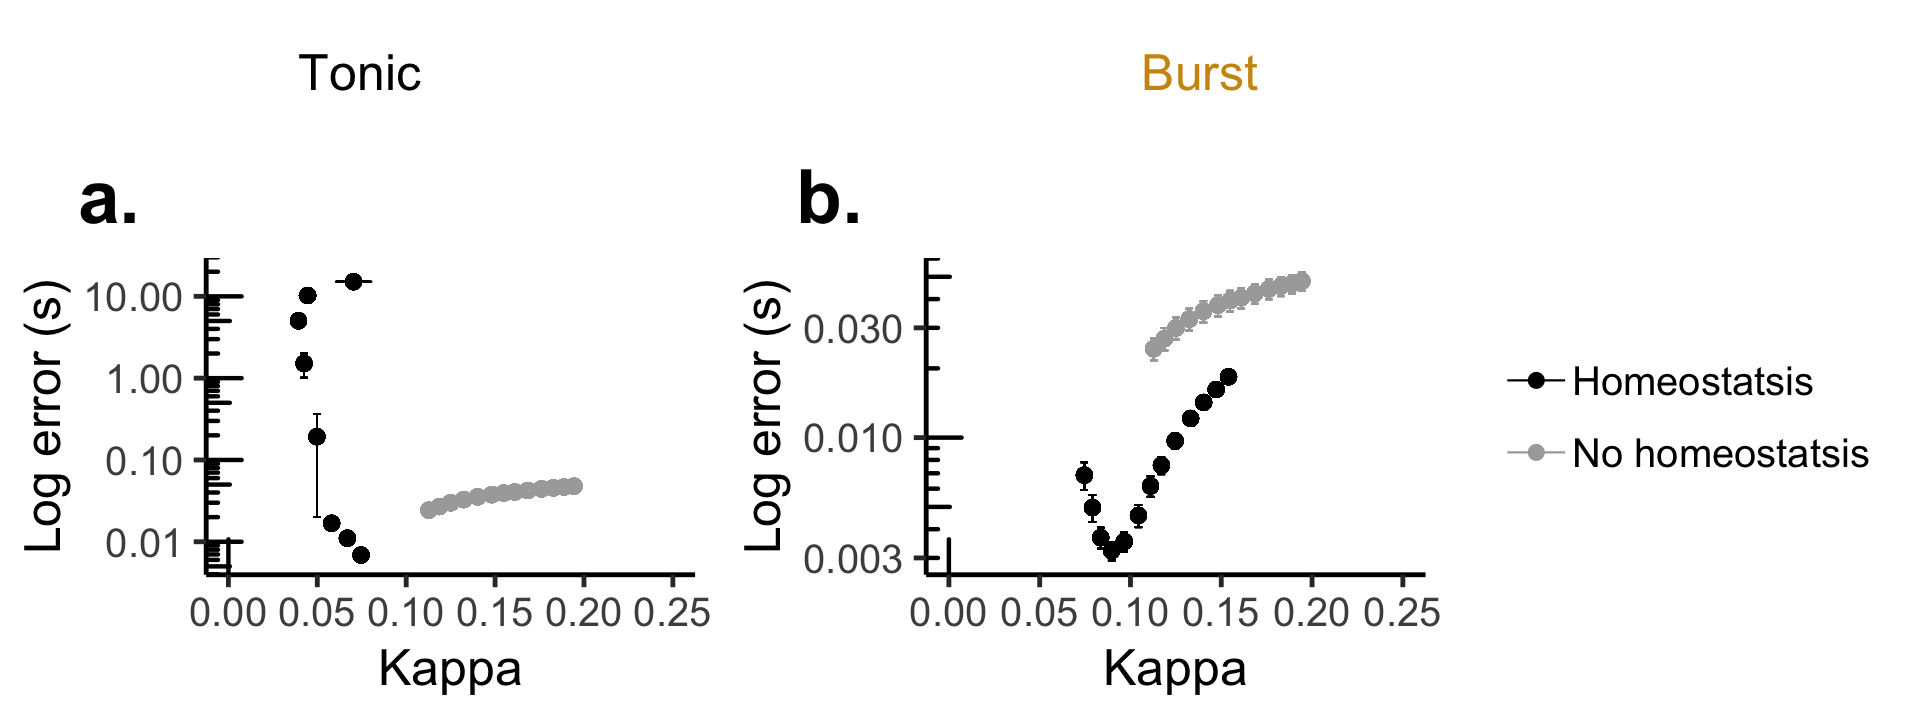
\includegraphics[width=0.6\textwidth]{fig3.png}
% \caption{\label{fig:f3}
%     Synchrony versus error during excitatory modulation, with (black) and without (grey) homeostasis.
%     \textbf{a.} Tonic modulation.
%     \textbf{b.} 4-cycle burst.
% }
% \end{figure}

% -----------------------------------------------------------------------
\subsection*{The effect of Ca\textsuperscript{2+} concentration.}
When the model is run with only stimulus-driven homeostasis, the Ca\textsuperscript{2+} concentration equilibrates to about 0.003 mM. We used this as a standard target value for all modulation experiments, until now. When we vary this value in 0.0002 mM increments, population rate and synchrony either increases or decreases depending on whether the Ca\textsuperscript{2+} increases or decreases, shown Figure \ref{fig:f4}\textbf{a-b}. However despite different initial Ca\textsuperscript{2+} concentrations, each model still shows an identical set of trends as the strength of the oscillation increases (Figure \ref{fig:f4}). That is, increasing or decreasing the target concentration shifts the overall excitability of the network, in an approximately linear way. This means that while the initial choice of 0.003 mM was arbitrary, the qualitative pattern of results we report is not dependent on this choice.

\begin{figure}
\centering
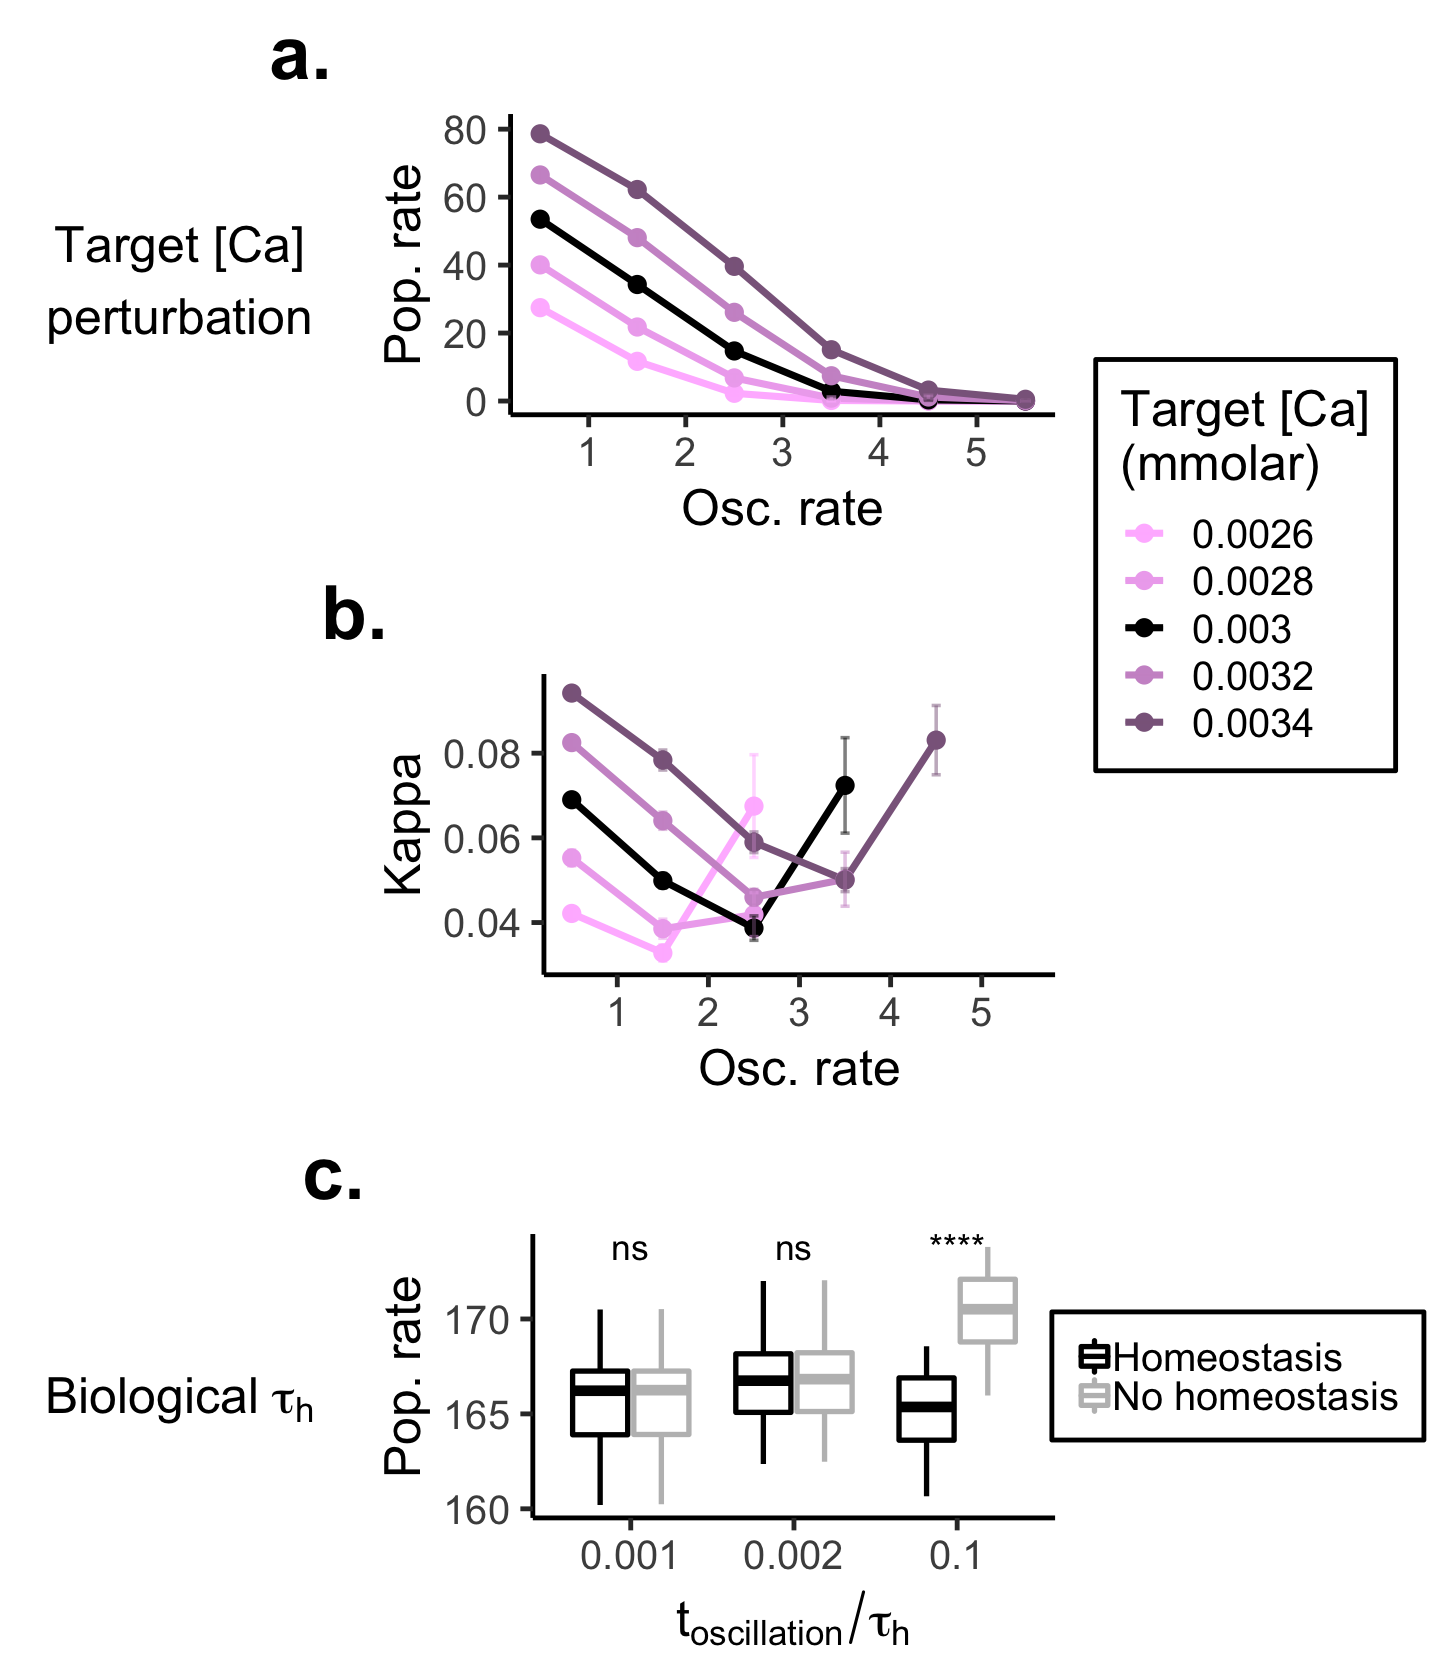
\includegraphics[width=0.5\textwidth]{fig4.png}
\caption{\label{fig:f4}
    Synchrony and excitability shift linearly with the target Calcium concentration, [Ca]. Plotted here is the effect of Ca\textsuperscript{2+} on a tonic excitatory modulation. The black value (0.003 mM) is the standard reference value used in all previous simulations.
    \textbf{a.} Change in population hippocampal population rate for different levels of target [Ca] (colors) as a function oscillation strength (Osc. rate on the x-axis). All values are referenced to a no-modulation control.
    \textbf{b.} Change in population synchrony for different levels of target [Ca] (colors) as a function oscillation strength (firing rate). All values are referenced to a no-modulation control.
    \textbf{c.} Change in population rate as the oscillation duration approaches a more realistic $\tau_h$, the half-life of the homeostasis dynamics (Eq.~\ref{eq:dgdt}). In this control experiment we used a more biologically realistic $\tau_h$ of 600 s (or 10 minutes). All other simulations in the report use a $\tau_h$ of 4 seconds, which is well below most reports of this value in real systems. However in choosing such as small value we follow the majority of the homeostasis modeling literature (for more on this see the \textit{Discussion}).
}
\end{figure}


% -----------------------------------------------------------------------
% -----------------------------------------------------------------------
% -----------------------------------------------------------------------
\section*{Discussion}
Our scientific understanding of homeostasis has been shaped as much by theoretical work as empirical \cite{Marder2014}. In an attempt to understand the interaction between oscillatory modulations and homeostasis, we begin by studying one of the simplest models used in early studies of homeostasis--a population of point neurons \cite{LeMasson1993}.

The feed-forward model of hippocampal pyramidal cells studied here serves as a simple initial model to answer three basic questions. One, do tonic oscillations--generated with biologically-consistent parameters--engage homeostatic mechanisms? Two, does homeostasis in turn change the oscillation's function? Three, do short bursts of oscillation have distinct effects from tonic oscillations? Put another way: can homeostasis help explain why some oscillations, such as hippocampal theta, tend to appear as tonic rhythms while other oscillations tend to appear as bursts? Our results suggest that homeostasis can explain why hippocampal theta is synaptically inhibitory, and why cortical oscillations often appear as bursts.

Bursting, rather than sustained, oscillations tend to be common in the cortex. One striking example is in motor cortical regions, where beta (~12-30 Hz) bursts are prevalent and likely functional. Specifically, beta bursts are very short--sometimes lasting only one or two cycles \cite{Sherman2016}--and relate to self-timed movements \cite{Feingold2015}. Patients with Parkinson's disease show increased motor rigidity and bradykinesia, symptoms associated with prolongation of beta bursts \cite{Tinkhauser2017}. Levodopa treatment was shown to decrease burst probability and duration, and that decrease in burst duration correlated with motor improvement \cite{Tinkhauser2017}.

While many neocortical oscillations tend to be bursty, a counterexample is visual cortical alpha, which can become tonic and high power when humans rest with their eyes closed. Even though both cortical and sub-cortical alpha generators are synaptically excitatory, this rhythm had been classically and paradoxically associated suppression of excitability \cite{Jensen2002,Bonnefond2012,Peterson2017}. While several competing explanations have been offered \cite{Bonnefond2012,Lange2013,Peterson2017} for this paradox, our work raises another possibility. Though we modelled hippocampal cells, the same Ca\textsuperscript{2+} homeostatic mechanisms exist in neocortex. Meaning strong and tonic alpha oscillations, combined with homeostasis, directly suppress population firing in visual cortex. Such an effect, were it to occur, would last well past the moment of oscillation offset. In fact, such long term effects of alpha have been reported in the literature, though the physiological mechanism was often unclear. Our work suggests that intrinsic homeostasis may underlie these effects.

\subsection*{Limitations}
The nature of our model--that fact we use point neurons with only 6 currents--or the fact that our model is strictly feed-forward--without lateral or recurrent connections--means we don't know with confidence to what degree our model's effects will appear in more complex models, or in real neural systems. For example, the primate or rat hippocampus. We do know, however, that oscillations are a ubiquitous feature of cortical activity, as is Ca\textsuperscript{2+}-mediated intrinsic homeostasis. This means the ingredients for oscillation and homeostasis to interact are omnipresent in both sub-cortical and cortical areas.

Homeostatic interactions depend on a number of factors specific to each cell and circuit. These include the duty cycle, power, and frequency of an oscillation, as well as on synaptic strengths and their location in the dendritic tree (an idea we return to below). It also depends on the other inputs into the cell, both from fast synaptic transmission and other (slower) modulators, as well a connection type; simulation studies suggest that recurrent connections can strongly interact with homeostatic regulation \cite{Harnack2015}. The temporal and spatial scales of these factors will strongly influence Ca\textsuperscript{2+} dynamics, which is in turn central to governing what, if any, homeostatic effects oscillations may generate.

Synaptic homeostasis may also play a role in tuning a neuron's response to all types of oscillatory perturbations, as both excitatory and inhibitory synapses are susceptible \cite{Cannon2016}, though in the case of excitatory modulation synaptic and intrinsic homeostasis appear to be linked \cite{Joseph2017}. Still, the exact nature of the response depends on how, and to what degree, oscillatory input and other sensory or internally driven ``computational'' inputs share synapses. This in turn requires considering complex dendritic arbors and their effect on homeostasis \cite{LeMasson1993}, neuromodulation \cite{Jadi2012,Jadi2014}, and computation \cite{Mainen1996,Polsky2004,Mel2004}. Considering these interacting effects together is the next step needed to develop a clearer biological understanding of modulatory oscillations. For inhibitory oscillations the case is even more complex: Ca\textsuperscript{2+} in these cells does not appear to regulate intrinsic homeostasis, but synaptic homeostasis is under a separate mechanism of control \cite{Joseph2017}.

\subsection*{Previous work}
Homeostasis has been extensively studied in the rhythmic pacemaker present in the crab stomatogastric ganglion. Here homeostasis has been shown to stabilize self-organized oscillations \cite{Golowasch1999}, and interact with neuromodulation in a \textit{highly} state dependent way \cite{Marder2014,Marder2015,Marder2014}. However, this work has focused on how chemical neuromodulators affect the formation of a pacemaker, not how a pacemaker can modulate another, downstream, circuit. Which is our focus here.

The interaction between homeostasis and oscillations has previously been considered when the oscillatory input is treated as a signal, not a modulator. Cannon and Miller \citep{Cannon2017} explored how synaptic homeostasis can effectively minimize the effect of modulatory perturbations, thus maximizing mutual information between an incoming oscillatory signal and a single cell's firing pattern. Our analysis could be considered an inverse complement to \citep{Cannon2017}--we study how to minimize the perturbation caused by a modulatory oscillator, rather than how to maximize the transmission of an oscillator.

\subsection*{Conclusion}
 Here, using a relatively simple model of hippocampal neurons, we observe a surprising--even paradoxical--result: that homeostatic effects can invert a normally synchronizing excitatory oscillatory neuromodulator and cause it to become inhibitory and desynchronizing.
 
 Based on our simple model, we conjecture that intrinsic homeostasis may explain why tonic theta rhythms in the hippocampus are synaptically inhibitory. To make this clear, consider the alternative. If the theta rhythm was strong, tonic, and synaptically excitatory, our model suggests this could lead to an equally strong--but opposing--homeostatic response. According to our model, such as response means that the firing threshold increases and the likelihood a hippocampal neuron can respond to any given stimulation would decrease, perhaps markedly so.

In effect, strong excitatory oscillations consume a substantial portion of each cell's possible dynamic range. On the other hand inhibitory oscillations do not generate an intrinsic homeostatic response, and so leave the dynamic range of the neurons intact. This may also explain why neocortical oscillations tend to be short and bursty, and why some neurological disorders, such as Parkinson's disease, are associated with prolonged rhythms.

% Computational modeling plays a critical role in neuroscience. Explicit computational modeling moves the field from "word model" theories to self-consistent mathematical formalizations [REF]. While these models can be wrong, they offer testable novel venues for research that are often difficult to find due to the immense complexity of the rich, dynamic neuronal environment.

\section*{Methods}
\subsection*{Mathematical model}
We model a feedforward network of hippocampal neurons, subjected to oscillatory modulation. This is instantiated as $N = 2000$ input cells connected to $M = 100$ Hodgkin-Huxley neurons. The $M$ cells in the network were tuned to mimic regular firing \cite{Borgers2005,Borgers2008}. The firing pattern of each input cell (both stimulus and modulation) is from a Poisson process, with a time-varying rate. $N_o$ cells oscillate. $N_s$ serve as input. For simplicity, we let $N_o = \frac{N}{2}$ so $N_o = N_s$. All input cells have a $p = 0.1$ connection probability to the hippocampal population. The synaptic weights for all $N \rightarrow M$ connections $w$ were independently sampled from a uniform distribution, $w \sim \mathcal{U}(5, 50)$ $\mu$S. The firing rate of the oscillating population was governed by sinusoidal pacemaker, with amplitude $A$ and frequency $f$, with the exact form $r_o / 2 (1 + \text{sin}(2 \pi f t)$. As a result, $r_o$ defines the peak firing of the oscillation. The stimulus population was simply modeled by a fixed rate of 6 Hz ($r_s$). The background firing rate $r_b$ was constant, and set at 2 Hz.

Hodgkin-Huxley dynamics were governed by 4 active ionic currents ($I_{Na}$, $I_{K}$, $I_{KCa}$, $I_{Ca}$) and the passive leak current ($I_l = g_l (E_l - V)$). Besides $I_{Ca}$ (which is discussed below), active currents are governed by the standard Hodgkin and Huxley form \cite{Hodgkin1952}. Where $m$ and $h$ respectively track the opening and closing channel kinetics, and $E$ is the channel appropriate Nernst reversal potential. See \textit{Table 1} for the complete set of parameters.

\begin{equation}
\label{eq:Idef}
I = \bar{g} m^p h^q (E - V)
\end{equation}

The Ca\textsuperscript{2+} current $I_{Ca}$ was governed by a form taken from the Morris-Lecar model \cite{Morris1981,LeMasson1993,Siegel1994}.

\begin{equation}
I_\text{Ca} = g_\text{Ca} [1 + \text{tanh} \Big ( \frac{V_1 - V}{ V_2} \Big ) (V_\text{Ca} - V)]
\end{equation}

Overall membrane dynamics were governed by these internal ion conductances, a variable bias current $I_\text{bias}$, and the excitatory synaptic input term $I_S$, which contains both background, stimulus, and oscillatory terms. All synaptic input was in turn governed a single exponential kinetics, which we denote generically using an $x$ subscript below. Though each synaptic input had different inputs, all models shared the same parameters. That is, $\tau_x = \tau_b = \tau_s = \tau_o$ and $\bar{g_x} = \bar{g_b} = \bar{g_s} = \bar{g_o}$.

\begin{equation}
    I_S = -g_b (E_s - V) + -g_s (E_s - V) + -g_o (E_o - V) 
\end{equation}
\begin{equation}
    \tau_x \frac{dg_x}{dt} = -g_x + \bar{g_x} \delta(t - t_x^j)
\end{equation}

\begin{equation}
C \frac{dV}{dt} = I_l + I_{Na} + I_{K} + I_{KCa} + I_{Ca} + I_{\text{bias}} + I_S
\end{equation}

The intrinsic excitability is regulated by altering both inward and outward conductances in response to changes in Ca\textsuperscript{2+} concentration. Following the previous work \cite{LeMasson1993} and \cite{Siegel1994}, we modeled this by allowing the maximal conductances $\bar{g_\text{Na}}$, $\bar{g_\text{K}}$, $\bar{g_\text{KCa}}$, and $\bar{g_\text{Ca}}$ to non-linearly vary in response to changes in Ca\textsuperscript{2+} concentration, $\text{Ca}$. During homeostatic equilibration, conductances drifted until the target Ca\textsuperscript{2+} concentration was met, denoted as $C_T$. In a control experiment a range of $C_T$ values were explored (Figure \ref{fig:f4}), though simulations defaulting to 0.03 mM; the value the system reaches with stimulation ($r_s = 6$ Hz) without modulation ($r_o = 0$). The $\pm$ symbol in equation \ref{eq:dgdt} denotes the direction of ion flow and is $(+)$ for inward going currents (Na and Ca) and $(-)$ for outward going Potassium.

\begin{equation}
\label{eq:dgdt}
\tau_h \frac{d \bar{g_x}}{dt} = \frac{G_x}{1 + e^{\pm (Ca - C_T)/\Delta}}
\end{equation}

Ca\textsuperscript{2+} dynamics were assumed to follow first order kinetics, driven by the Ca\textsuperscript{2+} influx current and clearance rate constant $k$. Values for both $\gamma$ and $k$ were taken from \cite{Liu1998}.

\begin{equation}
\frac{d\text{Ca}}{dt} = -k \text{Ca} - \gamma I_\text{Ca}
\end{equation}

% \subsection*{Estimating excitability, synchrony, and error}
\subsection*{Estimating excitability and synchrony}
We measure excitability by comparing average firing rate of all $M$ neurons in an experiment, with ($r_m$) and without modulation ($\bar{r}_m$). This accounts for any homeostatic drift driven only by the background noise:

\begin{align}
    \label{eq:excite}
    \Delta r = \bar{r}_m - r_m
\end{align}

We measure synchrony using $\kappa$, a binned measure of spiking covariance \cite{Wang1996}. Where $X(l) = 0 \ \text{or} \ 1$ and $Y(l) = 0 \ \text{or} \ 1$ for $l = \{1, 2, ..., K \}$ and with $T/K = \tau$.

\begin{align}
    \label{eq:kappa}
    \kappa_{ij}(\tau) = \frac{\sum_l^K X(l)Y(l)}{\sqrt{\sum_l^K X(l) \sum_l^k Y(l)}}
\end{align}

\begin{align}
\kappa(\tau) = \frac{1}{N} \sum_i^N \sum_j^N \kappa(\tau)_{ij}
\end{align}

% Modulation is optional. Each of the different modulatory systems--oscillations, dopamine, and acetylcholine--to name a few among dozens of options, may be absent, weakly present, or operating at high level at any given moment of time. We therefore reason it is important to quantify how coding is perturbed under varying levels of modulation and homeostasis. We estimate this by comparing differences in spike timing between an experimental condition and a control run with without modulation. 

% Deviations in spike-timing caused by modulation are treated as errors, which we quantify with the mean squared error (Eq.~\ref{eq:error}). The more efficient a modulation, the less error it should introduce for a given change in either excitability or synchrony.  

% \begin{equation}
% \label{eq:error}
% \text{MSE} = \frac{1}{K} \sum_{i=1}^k (\hat{y} - y_i)^2
% \end{equation}

% In its mathematical form the MSE assumes the reference $\hat{t}$ and observed variables $y$ to be the same length. Here this constraint could not be satisfied: as $r_o$ increases, new action potentials are inevitable. To accommodate potentially ragged lengths we truncated the longer of the two series to match the shorter. For example, if the target series has length $K$, and the observed sequence has length $L$, when $K > L$ then $K-L$ elements are removed, starting with the largest value. When $L > K$, $L - K$ of the largest were eliminated. 

% -------------------------------------
\newpage
\begin{table}
\centering
\begin{tabular}{@{}lll@{}}
\toprule
\textbf{Symbol} & \textbf{Range (unit)} & \textbf{Description} \\ \midrule
$f$ & 8 (Hz) & Oscillation frequency \\
$r_o$ & 0 - 6 (Hz) & Oscillation firing rate \\
$r_s$ & 6 (Hz) & Stimulus firing rate \\
$C$ & 1 ($\mu$F) & Membrane capacitance \\
$\tau_h$ & \textgreater 4 (sec) & Homeostasis time constant \\
$w$ & 5 - 50 ($\mu$S) & Synaptic weight \\
$\tau_e$ & 5 (msec) & Excitatory synaptic time constant \\
$V_e$ & 0 (mV) & Excitatory synaptic reversal potential \\
$p$ & 0.1 & Connection probability \\
$C_T$ & 0.0028-0.0032 (mM) & Target Ca\textsuperscript{2+} concentration \\
$G_\text{Na}$ & 360 ($\mu$S) & Initial Na conductance \\
$G_\text{K}$ & 120 ($\mu$S) & Initial K conductance \\
$G_\text{KCa}$ & 60 ($\mu$S) & KCa conductance \\
$g_\text{Na}$ & 180 ($\mu$S) & Max. Na conductance \\
$g_\text{K}$ & 60 ($\mu$S) & Max. K conductance \\
$g_\text{KCa}$ & 30 ($\mu$S) & Max. K conductance \\
$g_\text{Ca}$ & 0.03 ($\mu$S) & Max. Ca\textsuperscript{2+} conductance \\
$g_l$ & 1 ($\mu$S) & Leak conductance \\
$V_l$ & -70 (mV) & Leak reversal potential \\
$V_K$ & -100 (mV) & K reversal potential \\
$V_\text{Na}$ & 50 (mV) & Na reversal potential \\
$V_\text{Ca}$ & 150 (mV) & Ca\textsuperscript{2+} reversal potential \\
$V_\text{1}$ & -50 (mV) & Morris-Lecar constant \\
$V_\text{2}$ & 10 (mV) & Morris-Lecar constant \\
$\Delta$ & 0.6 ($\mu$M) & Ca\textsuperscript{2+} influx rate \\
$k$ & 1/200 (1 / msec) & Ca\textsuperscript{2+} clearance rate \\
$\gamma$ & -0.00047 (mM / mA / msec) & Ca\textsuperscript{2+} current conversion constant \\
$\delta t$ & 0.01 (msec) & Integration time step \\ \bottomrule
\end{tabular}
\caption{Model parameters.}
\label{table:params}
\end{table}

% -----------------------------------------------
\newpage
\bibliography{library_min}

% -----------------------------------------------
\end{document}
